\documentclass[
    11pt, % Set the default font size, options include: 8pt, 9pt, 10pt, 11pt, 12pt, 14pt, 17pt, 20pt
    %
    aspectratio=169, % Uncomment to set the aspect ratio to a 16:9 ratio which matches the aspect ratio of 1080p and 4K screens and projectors
]{beamer}

\graphicspath{{Images/}{./}} % Specifies where to look for included images (trailing slash required)
\usepackage{booktabs} % Allows the use of \toprule, \midrule and \bottomrule for better rules in tables

%\usepackage{appendixnumberbeamer} %If you want a separate slide counter for your appendix

%%% Customize Theme %%%%%%%%%%%%%%%%%%%%%%
\usetheme{Madrid} % You can use other themes too, but this changes many things. I've found Madrid to be the best for this color scheme

%fg = font color
%bg = background color

% ! WARNING ! : Many colors are linked to multiple attributes, so changing one color can have unexpected changes!

% If you want to tweak the shading of orange and red, tweak the below 2 lines:t
\definecolor{myRed}{RGB}{120,4,4}
\definecolor{myOrange}{RGB}{227, 125, 0}

% Bottom right hand color
\setbeamercolor*{structure}{bg=myRed!20,fg=myRed!90}

\setbeamercolor*{palette primary}{use=structure,fg=white,bg=structure.fg} %?
\setbeamercolor*{palette secondary}{use=structure,fg=myRed,bg=white}
    %bottom left of footer & bar between title & top bubbles
\setbeamercolor*{palette tertiary}{use=structure,fg=white,bg=myRed} 

\setbeamercolor{frametitle}{bg=myRed!85,fg=white} %title of each slide

\setbeamercolor*{titlelike}{parent=palette primary} %?
%\setbeamercolor{titlelike}{parent=palette primary,fg=structure.fg!50!myRed}

%for miniframe (very top) AND center footer
\setbeamercolor{section in head/foot}{fg=myOrange, bg=white}

%%% Specific Colors %%%
\setbeamercolor{item projected}{bg=myOrange}
\setbeamertemplate{enumerate items}{bg=myOrange}

\setbeamercolor{itemize item}{fg=myOrange}
\setbeamercolor{itemize subitem}{fg=myOrange}

\setbeamercolor{button}{bg=myOrange}

%%% Edits ONLY the TOC slide %%%
\setbeamercolor{section in toc}{fg=black}
\setbeamercolor{subsection in toc}{fg=black}

%%% Block Colors %%%
% Standard block %
    \setbeamercolor{block title}{bg=myOrange, fg=white}
    \setbeamercolor{block body}{bg=myOrange!20}

% Alerted block % If you want to customize it's color
    %\setbeamercolor{block title alerted}{bg=cyan, fg=white}
    %\setbeamercolor{block body alerted}{bg=cyan!10}

% Example block % If you want to customize it's color
    %\setbeamercolor{block title example}{bg=cyan, fg=white}
    %\setbeamercolor{block body example}{bg=cyan!10}

%---------------------------------------------------------
%	SELECT FONT THEME & FONTS
%---------------------------------------------------------
\usefonttheme{default} % Typeset using the default sans serif font
\usepackage{palatino} % Use the Palatino font for serif text
\usepackage[default]{opensans} % Use the Open Sans font for sans serif text
\useinnertheme{circles}

%---------------------------------------------------------
%	SELECT OUTER THEME
%---------------------------------------------------------
% Outer themes change the overall layout of slides, such as: header and footer lines, sidebars and slide titles. Uncomment each theme in turn to see what changes it makes to your presentation.

%\useoutertheme{default}
%
\useoutertheme{miniframes}

%\useoutertheme{infolines}
%\useoutertheme{smoothbars}
%\useoutertheme{sidebar}
%\useoutertheme{split}
%\useoutertheme{shadow}
%\useoutertheme{tree}
%\useoutertheme{smoothtree}

%---------------------------------------------------------
%	PRESENTATION INFORMATION
%---------------------------------------------------------

\title{The Heartbleed Vulnerability}
\author{Authors: Adina-Maria VAMAN, Dragoș IOANA}
\logo{
\includegraphics[width=3cm]{heartbleed.png}}
\date[\today]

%---------------------------------------------------------
%---------------------------------------------------------
%---------------------------------------------------------
\begin{document}

%---------------------------------------------------------
%	TITLE SLIDE
%---------------------------------------------------------
\section{}
\begin{frame}
	\titlepage % Output the title slide, automatically created using the text entered in the PRESENTATION INFORMATION block above
\end{frame}

%---------------------------------------------------------
%	TABLE OF CONTENTS SLIDE
%---------------------------------------------------------
% The table of contents outputs the sections and subsections that appear in your presentation, specified with the standard \section and \subsection commands. You may either display all sections and subsections on one slide with \tableofcontents, or display each section at a time on subsequent slides with \tableofcontents[pausesections]. The latter is useful if you want to step through each section and mention what you will discuss.

\begin{frame}
	\frametitle{Table of Contents} % Slide title, remove this command for no title
	
	\tableofcontents % Output the table of contents (all sections on one slide)
	%\tableofcontents[pausesections] % Output the table of contents (break sections up across separate slides)
\end{frame}

%---------------------------------------------------------
%	PRESENTATION BODY SLIDES
%---------------------------------------------------------
\section{Background} % Sections are added in order to organize your presentation into discrete blocks, all sections and subsections are automatically output to the table of contents as an overview of the talk but NOT output in the presentation as separate slides

%------------------------------------------------
\begin{frame}
	\frametitle{OpenSSL}
            \begin{itemize}
                \item a popular open-source cryptographic library that implements the SSL and TLS protocols
                \newline
                \item it is widely used by server software to facilitate secure \newline connections for web, email, VPN, and messaging services
                \newline
                \item it was integrated in popular server products such as \emph{Apache} \newline and \emph{Nginx}
            \end{itemize}
\end{frame}

%------------------------------------------------
\begin{frame}
	\frametitle{Datagram Transport Layer Security}
	
	% Look at the code of this slide to see how columns made this formatting look nice.

	% \begin{columns}[t] % The "c" option specifies centered vertical alignment while the "t" option is used for top vertical alignment
	% 	\begin{column}{0.5\textwidth} % Right column width
 %                \begin{figure}[h!]
 %                    \centering
 %                    %\caption{Hawkins et al, 2015}
 %                    
\includegraphics[angle=0, width=4.5cm]{Hokie2.png}
 %                    %\label{Figure 1}
 %                \end{figure}
	% 	\end{column}
 %  		\begin{column}{0.5\textwidth} % Left column width
 %                \begin{figure}[h!]
 %                    \centering
 %                    %\caption{Hawkins et al, 2015}
 %                    
\includegraphics[angle=0, width=4.5cm]{Hokie2.png}
 %                    %\label{Figure 1}
 %                \end{figure}
	% 	\end{column}		
	% \end{columns}

        \begin{itemize}
            \item usually, TLS must run over a reliable transport channel - typically TCP
            \newline
            \item RFC6347 introduced \emph{Datagram Transport Layer Security Version 1.2}, \newline which aims to secure unreliable datagram traffic for application \newline layer protocols that are designed to use UDP transport 
            \newline
            \item standard implementations of TLS rely on TCP for session \newline management which UDP lacks - the need for \emph{TLS Heartbeat Extension}
        \end{itemize}
    
 
\end{frame}

%------------------------------------------------
\begin{frame}
	\frametitle{TLS Heartbeat Extension}
            \begin{columns}[t] % The "c" option specifies centered vertical alignment while the "t" option is used for top vertical alignment
		\begin{column}{0.5\textwidth} % Right column width
                \begin{figure}[h!]
                    \centering
                    \caption{Heartbeat package}
                    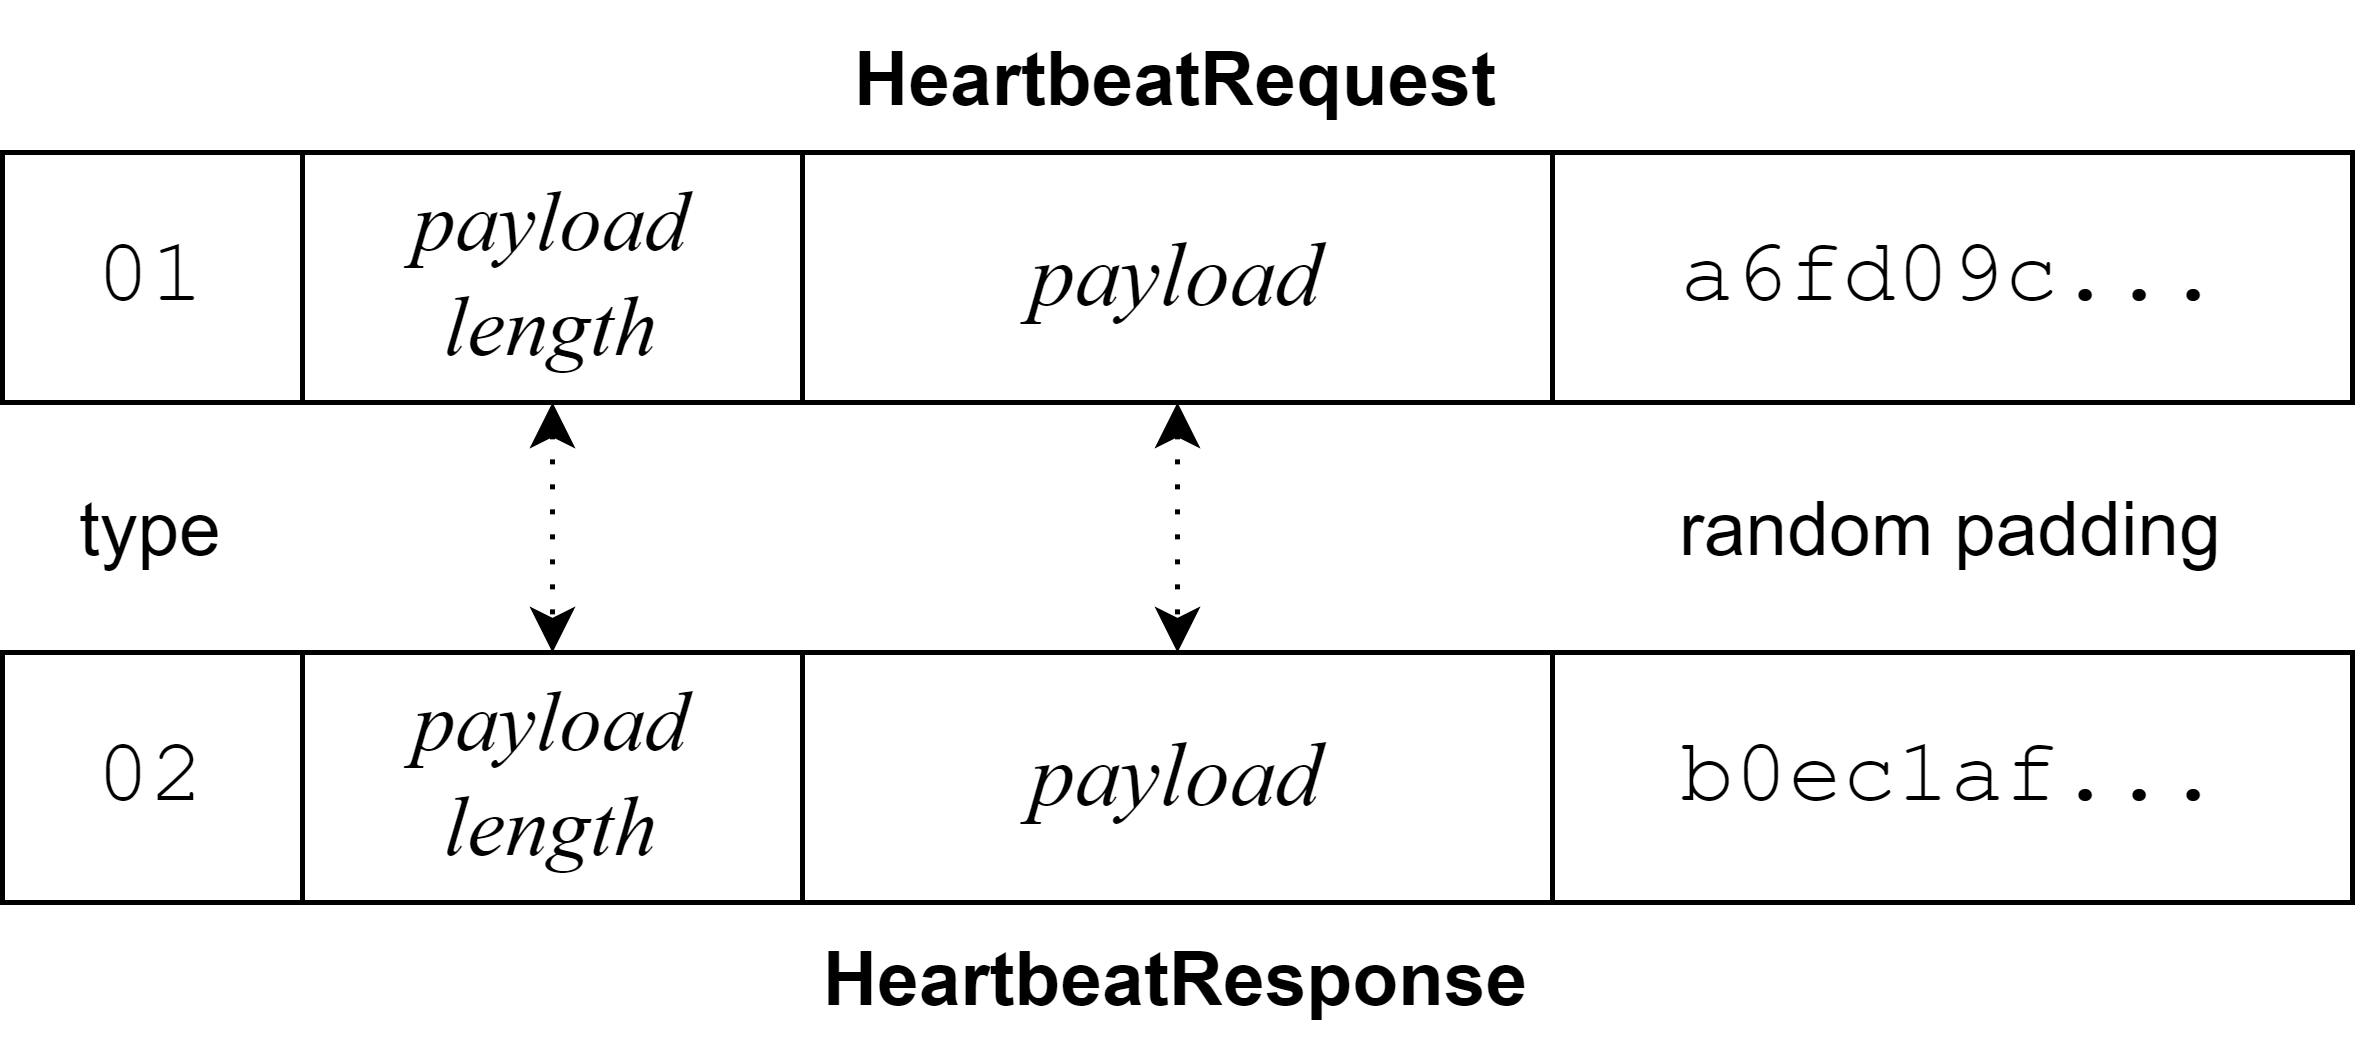
\includegraphics[angle=0, width=8cm]{Images/heartbeat-packet.png}
                    \label{Heartbeat package}
                \end{figure}
		\end{column}
  		\begin{column}{0.5\textwidth} % Left column width
                \newline
                \begin{itemize}
                \item allows either endpoint of a TLS connection to detect whether its peer is still present
                \newline
                \newline
                \newline
                \newline
                \item either endpoint can \newline send a HeartbeatRequest \newline message to verify connectivity
            \end{itemize}
		\end{column}		
	\end{columns}
\end{frame}

%------------------------------------------------
\section{The Heartbleed vulnerability}

%------------------------------------------------
\begin{frame}
\label{Test Stat}
	\frametitle{The Heartbleed vulnerability}
		\begin{figure}[h!]
            \centering
            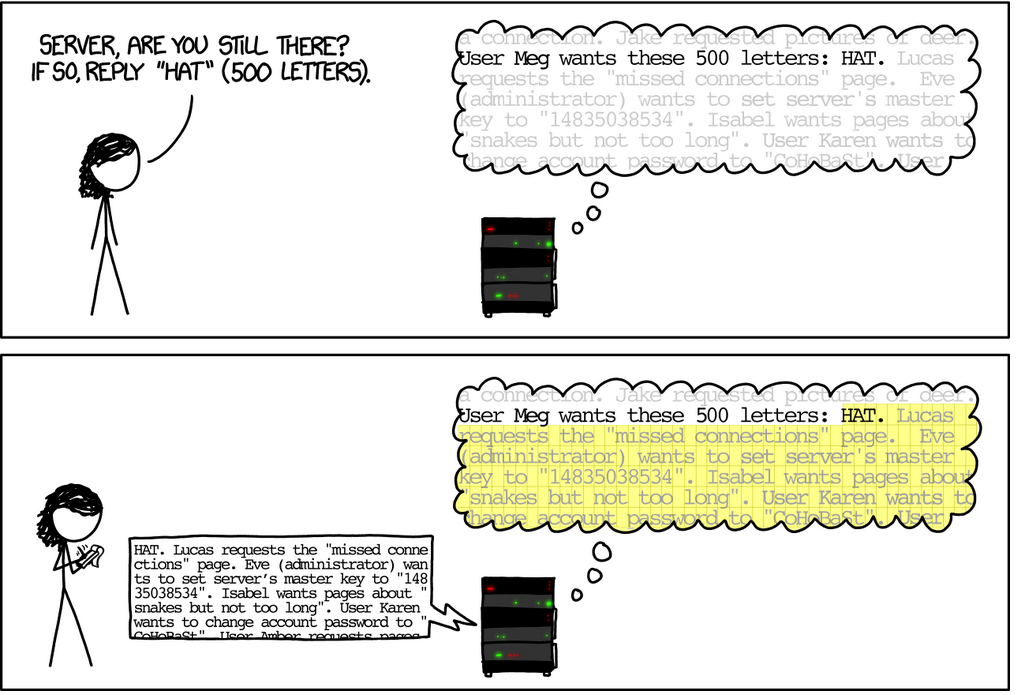
\includegraphics[angle=0, width=9cm]{xkcd.png}
            \label{Heartbleed}
        \end{figure}
\end{frame}
%------------------------------------------------
\begin{frame}
	\frametitle{The Heartbleed vulnerability}
            \begin{itemize}
                \item it allows either end-point to read data
following the payload message in its peer’s memory by specifying a payload length larger than the amount of data in the \emph{HeartbeatRequest} message
\newline
\newline
\newline
                \item  Because the payload length field is two bytes, the peer responds \newline with up to 216 bytes (around 64 KB) of memory
            \end{itemize}
\end{frame}


%------------------------------------------------
\begin{frame}
	\frametitle{Timeline}
            \begin{itemize}
                \item 03/21 Neel Mehta of Google discovers Heartbleed
                \item 03/21 Google patches OpenSSL on their servers
                \item 03/31 CloudFlare is privately notified and patches
                \item 04/01 Google notifies the OpenSSL core team
                \item 04/02 Codenomicon independently discovers Heartbleed
                \item 04/03 Codenomicon informs NCSC-FI
                \item 04/04 Akamai is privately notified and patches
                \item 04/05 Codenomicon purchases the heartbleed.com domain
                \item 04/07 NCSC-FI notifies OpenSSL core team
                \item 04/07 OpenSSL releases version 1.0.1g and a security advisory
            \end{itemize}
\end{frame}

%------------------------------------------------
\begin{frame}
	\frametitle{Impact}
            \begin{itemize}
                \item it may have affected any service that used OpenSSL to facilitate TLS connections
                \newline
                \newline
                \item any type of confidential data could have been exposed:
                \newline
                    \begin{itemize}
                        \item session cookies
                        \item private keys
                        \item server master keys
                        \item authentication material
                    \end{itemize}
            \end{itemize}
\end{frame}

%------------------------------------------------
\begin{frame}
	\frametitle{Mitigation}
            \begin{itemize}
                \item \emph{patching OpenSSL to a version $\geq$1.0.1g}
                \newline
                \item changing passwords
                \newline
                \item regenerating key pairs
                \newline
                \item revoking old certificates
                \newline
                \item deleting cookies
                \newline
                \item compiling OpenSSL sources with \emph{-DOPENSSL\_NO\_HEARTBEATS} flag
            \end{itemize}
\end{frame}

%------------------------------------------------
\section{Proof of Concept}

%------------------------------------------------
\begin{frame}
	\frametitle{PoC description and implementation}
 Exploit architecture:
        \begin{itemize}
            \item vulnerable Apache server using OpenSSL v1.0.1e which exposes an HTML page that saves login data as cookies
            \newline
            \newline
            \newline
            \item exploit script as source code in C, which does the TLS Handshake \newline and then requests Heartbeat responses to look for server echoing \newline back sensitive information
        \end{itemize}
    	% \begin{block}{Block Title}
    	% 	Block 1
    	% \end{block}
    	
    	% \begin{exampleblock}{Example Block Title}
    	% 	Block 2
    	% \end{exampleblock}
    	
    	% \begin{alertblock}{Alert Block Title}
    	% 	Block 3
    	% \end{alertblock}
    	
    	% \begin{block}{} % Block without title
    	% 	Block without a title
    	% \end{block}
\end{frame}

%------------------------------------------------
\begin{frame}
	\frametitle{PoC description and implementation}
           \begin{center}
               \large\emph{Live demo}
           \end{center} 
\end{frame}

\end{document} 